\chapter{Resultados}
Neste capítulo serão apresentados os resultados obtidos pelo algoritmo Pollard-rho e suas variações juntamente com a descrição dos parâmetros utilizados.

\section{Descrição dos experimentos}
\begin{enumerate}

\item Implementar os seguintes algoritmos para solucionar o problema do logaritmo discreto para curvas elípticas:
  \begin{itemize}
  \item Pollard-rho com único processador.
  \item Pollard-rho com paralelização.
  \item Pollard-rho com múltiplos processadores.
  \end{itemize}
\item Escolher curvas e seus parâmetros cuja criptografia possa ser ``quebrada'' em um tempo adequado para que as comparações entre os diversos algoritmos possam ser realizadas.
\item Escolher pontos \(P\) e \(Q\) pertencentes à curva e elaborar o problema do logaritmo discreto.
\item Solucionar o problema utilizando os algoritmos implementados.
\item Verificar o tempo de execução necessário para cada algoritmo resolver o problema.
\item Comparar o tempo de execução dos algoritmos entre si.
\item Comparar o desempenho do Pollard-rho multi processado para diferentes quantidades de processadores.
% \item Verificar se os resultados obtidos condizem com os resultados esperados de acordo com a bibliografia pesquisada.

\end{enumerate}

\section{Escolha das curvas}
As curvas escolhidas para a execução dos testes foram geradas com o auxílio da biblioteca SageMath. Quanto aos parâmetros, foi escolhido um número primo \(p\) para representar o corpo finito no qual a curva está definida. Os parâmetros \(a\) e \(b\) foram selecionados seguindo a regra estabelecida na Equação \ref{eq:7}. Após isso, foi feito o cálculo da ordem da curva, se a ordem é prima, a curva é utilizada, caso contrário, será descartada e outra curva será gerada seguindo os mesmos passos citados, até que seja encontrada uma curva com a ordem prima. Dessa forma, pode-se evitar ataques baseados na fatoração da ordem da curva, tais como o ataque utilizando o algoritmo de Pohlig-Hellman (Seção \ref{sec:algs}).

Gerou-se diferentes curvas variando o valor de \(p\) de 32 a 160 bits para, posteriormente, realizar a comparação de tempo entre os algoritmos. Foram também selecionados dois pontos \(P\) e \(Q\) pertencentes à curva. Por fim, todas essas informações foram armazenadas em um arquivo de texto para ser processado pelos algoritmos.

\section{Implementação e execução dos algoritmos}

\subsection{Pollard-rho serial}
Para realizar a implementação do Pollard-rho com único processador (serial) seguiu-se a descrição do pseudo-algoritmo no Anexo \ref{alg:single} juntamente com a teoria explanada na Seção \ref{sec:single}. O ponto inicial foi escolhido de forma arbitrária para cada vez que o algoritmo fosse executado e foi utilizado apenas um processador, pois esta abordagem não possui suporte à paralelização.

A maior vantagem desse algoritmo é que ele necessita de uma quantidade ínfima de memória, pois utiliza o ciclo de Floyd, descrito na seção \ref{floyd}. Dessa forma, este algoritmo pode ficar executando por tempo indeterminado mesmo em uma máquina com pouca memória.

\subsection{Pollard-rho com paralelização}
Buscando aproveitar a baixa quantidade de memória utilizada pelo Pollard-rho serial, e diminuir o tempo necessário para resolver o problema do logaritmo discreto, foi implementada uma versão modificada do algoritmo serial para que o código pudesse executar de forma paralela, afim de poder utilizar todos os processadores disponíveis da máquina. Por isso, este algoritmo difere do algoritmo serial apenas do ponto de vista estatístico.

Basicamente são utilizados \(M\) núcleos (virtuais) em que cada um executa um processo rodando o algoritmo Pollard-rho de forma independente, com diferentes pontos iniciais \(X_0\) aleatórios, enquanto o algoritmo serial seleciona apenas um ponto inicial. Por mais que esta abordagem não seja a mais eficiente em termos de tempo execução, essa medida obteve melhorias, as quais serão apresentados na Seção \ref{sec:execution_time}.

\subsection{Pollard-rho com múltiplos processadores}
O algoritmo mais eficiente é o Pollard-rho com múltiplos processadores (multiprocessado), pois este é diferente em relação aos outros algoritmos quanto à técnica e o tempo esperado de processamento, de acordo com a Seção \ref{sec:parallelized}. A utilização de um servidor central para o armazenamento de pontos é o ponto positivo do algoritmo, pois o processo que calcula os pontos ganha em velocidade por não ter a responsabilidade de checar a colisão entre os pontos e também por evitar a necessidade de um recurso compartilhado entre os processos, já que o servidor central é o único responsável por armazenar e checar a colisão entre os pontos.

O ponto negativo dessa abordagem é que o servidor não pode armazenar infinitos pontos, pois existe o limite da memória RAM. Para isso utilizou-se a propriedade distintiva (Seção \ref{sec:distinguished}), que vai limitar a quantidade de pontos que o servidor irá armazenar. Porém, caso essa propriedade seja muito restritiva, a possibilidade de encontrar uma colisão diminui, pois o servidor central terá um espaço amostral de pontos menor para encontrar uma colisão e, consequentemente, o tempo de execução do algoritmo irá aumentar. Por outro lado, caso a propriedade for muito abrangente, a memória pode esgotar rapidamente. Dessa forma, é necessário encontrar um equilíbrio para essa propriedade distintiva, pois quanto mais abrangente, maior a quantidade de memória utilizada para armazenar os pontos, quanto mais restritiva, menor a quantidade de pontos armazenados e maior o tempo para encontrar uma colisão entre estes pontos.

Durante a execução desse algoritmo, foram feitos diversos testes sobre a utilização da propriedade distintiva mais adequada até chegar a uma que fosse considerada boa. A propriedade escolhida foi o \textit{Hamming weight} da coordenada x do ponto ser menor que 24. Além da dificuldade inerente a essa propriedade, ficou evidente também o problema de memória RAM, pois, apesar da utilização de uma propriedade distintiva para armazenar os pontos (o que diminui o número de pontos a serem armazenados), 16GB de memória se tornavam insuficientes após aproximadamente 25 horas de execução do algoritmo, resultando em falta de memória a partir de uma curva de 66 bits.

\section{Tempo de execução}
\label{sec:execution_time}

\begin{table}[h]
\centering
\label{table:results}
\begin{tabular}{|l|c|c|c|}
\hline
\rowcolor[gray]{0.9}
\multicolumn{1}{|c|}{\(bits\)} & \textbf{Serial} & \textbf{Paralelizado} & \textbf{Multiprocessado} \\ \hline
32                             & 0h00m01s        & 0h00m01s              & 0h00m01s                 \\ \hline
36                             & 0h00m08s        & 0h00m04s              & 0h00m01s                 \\ \hline
40                             & 0h00m46s        & 0h00m19s              & 0h00m03s                 \\ \hline
44                             & 0h02m58s        & 0h01m26s              & 0h00m14s                 \\ \hline
48                             & 0h17m11s        & 0h14m47s              & 0h01m04s                 \\ \hline
52                             & 0h20m26s        & 0h16m49s              & 0h04m54s                 \\ \hline
56                             & 1h27m28s        & 2h46m18s              & 0h29m12s                 \\ \hline
60                             & 15h11m05s       & 8h56m45s              & 0h41m38s                 \\ \hline
64                             & 2d 14h37m58s    & 1d 15h52m12s          & 6h44m23s                 \\ \hline
65                             & 3d 20h45m48s    & -                     & 10h33m34s                \\ \hline
66                             & 6d 04h30m10s    & -                     & -                        \\ \hline
\end{tabular}
\caption{Resultado dos algoritmos Pollard-rho}
\end{table}

Com os experimentos realizados durante este trabalho, foi possível realizar uma comparação empírica entre três variantes do algoritmo Pollard-rho para ataques à criptografia de curvas elípticas. Assim, foi possível verificar os pontos fortes e as fragilidades que cada uma das abordagens oferece, bem como verificar na prática a dificuldade computacional para resolver o problema do logaritmo discreto.

Os resultados apresentados na tabela \ref{table:results} demonstram que utilizar múltiplos processos para a solução do problema é a abordagem que oferece um desempenho melhor caso seja levado em consideração apenas o tempo de execução do algoritmo. Já em contrapartida, essa abordagem traz uma preocupante restrição física para sua implementação, que é a quantidade de memória necessária para a realização dos experimentos.

Para amenizar esse problema, foi utilizado uma propriedade distintiva que seleciona os pontos que devem ser armazenados na memória, descartando todos os outros pontos que não atendiam tal propriedade. A escolha dessa propriedade distintiva oferece um \textit{trade-off} inevitável, pois, caso seja selecionada uma propriedade muito restritiva, a quantidade de pontos armazenados será significativamente menor, aumentando o ``tempo de vida'' da memória e permitindo que o algoritmo seja executado por mais tempo. Porém, ao restringir muito a quantidade de pontos armazenados, o espaço amostral que o algoritmo dispõe para encontrar uma colisão é menor, e portanto, será necessário mais processamento para encontrar uma colisão e, consequentemente, o tempo necessário para resolver o problema do logaritmo discreto será maior. Diante desse \textit{trade-off}, pode-se verificar a importância da escolha dessa propriedade distintiva, algo que necessita e merece mais pesquisas por parte da comunidade acadêmica.

Já os algoritmos Pollard-rho serial e paralelo não possuem o problema da memória que a versão com múltiplos processadores apresenta. A vantagem desses algoritmos é utilizar sempre a mesma quantidade de memória para os cálculos, ou seja, o consumo de memória será sempre o mesmo durante toda a execução do algoritmo. Porém, é possível perceber pela tabela \ref{table:results} que esses algoritmos são mais lentos para resolver o problema do logaritmo discreto.

A melhoria de desempenho do algoritmo paralelo em relação ao serial é justificada por uma questão estatística, pois o algoritmo serial escolhe um ponto inicial de forma aleatória, e dependendo dessa escolha, o algoritmo pode demorar mais tempo para encontrar uma colisão. Já na versão paralelizada, o mesmo algoritmo serial é executado em paralelo por vários processos, onde cada um deles é inicializado com um ponto inicial. Dessa forma, um desses processos vai partir de um ponto inicial mais propício a encontrar uma colisão do que os outros processos e, consequentemente, este processo irá encontrar uma colisão em um tempo menor do que os outros.

Os resultados da tabela \ref{table:results} podem ser colocados em um gráfico \textit{Mono-Log}, onde a coordenada $x$ do gráfico representa o tamanho da curva em \textit{bits} e a coordenada $y$ representa o tempo, em segundos, necessário para resolver o problema do logaritmo discreto. O resultado é o gráfico da figura \ref{grafico1}.

Pelo gráfico da figura \ref{grafico1} é possível perceber que os resultados experimentais se aproximam de uma reta. Isto demonstra que pode-se obter uma função que irá calcular o tempo aproximado para resolver o problema do logaritmo discreto partindo do tamanho da curva em bits, e que esta função é exponencial do tipo \(y = ke^{cx}\), onde $e$ é a base dos logaritmos neperianos.

\begin{figure}[h]
\centering
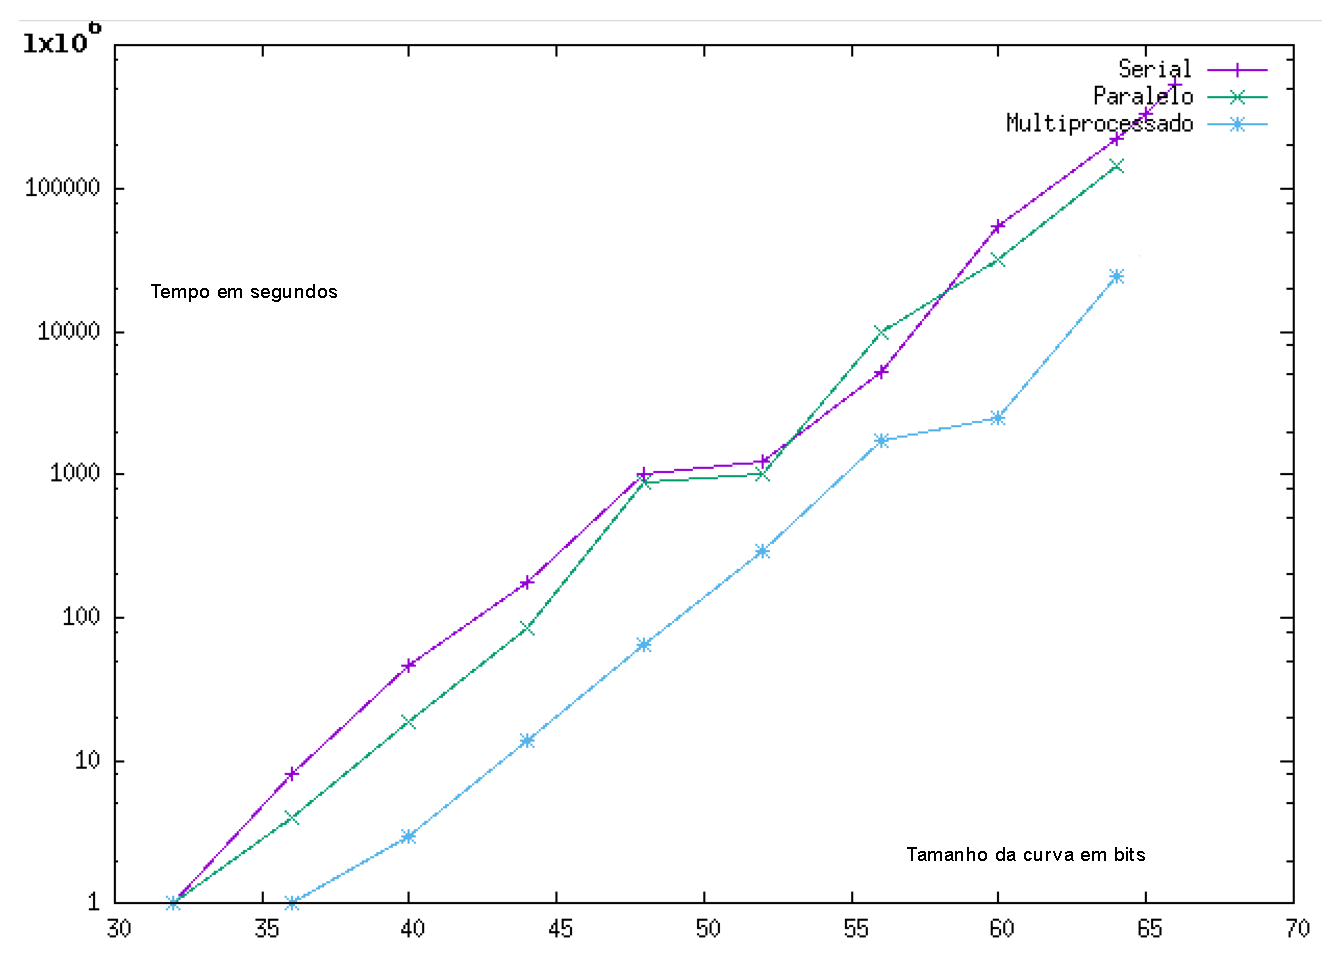
\includegraphics[scale=0.6, bb=0 0 515 478]{figuras/grafico1.eps}
\caption{Tamanho em \textit{bits} X Tempo em segundos (escala logarítmica)}
\label{grafico1}
\end{figure}

Para obter a equação que relacione o tempo necessário em segundos para ``quebrar'' uma curva de $n$ bits, foi aplicada a função \(ln(x)\) em ambos os lados da equação \(y = ke^{cx}\), obtendo-se
\begin{equation} \label{eq_linear}
	ln(y) = ln(k) + cx\cdot ln(e) = ln(k) + cx
\end{equation}
Em seguida, foram escolhidos dois pontos \(A\) e \(B\) de uma das curvas do gráfico \ref{grafico1}, e substituidos os valores de \(x\) e \(y\) na equação (\ref{eq_linear}) respectivamente pelas coordenadas de \(A\) e \(B\), obtendo-se o sistema
\begin{equation*}
\left\{ \begin{array}{c}
ln(Y_A) = ln(a) + b(X_A)\\
ln(Y_B) = ln(a) + b(X_B)
\end{array}
\right.
\end{equation*}

Com esse sistema, ao fazer \(ln(Y_B) - ln(Y_A)\), obtém-se o valor de \(b\), e em seguida o valor de \(ln(a)\). Por último, aplica-se a função exponencial de ambos os lados da equação \(ln(y) = ln(a) + bx\) resultante, com os valores de \(ln(a)\) e de \(b\) já substituídos. O resultado é uma equação do tipo
\begin{equation*}
	y = e^{ln(a) + bx}
\end{equation*}
onde \(e \approx 2.718281828\).

Dessa forma, as equações que relacionam o tamanho da curva em \textit{bits} ao tempo necessário em segundos para ``quebrá-la'' foram as seguintes
\begin{itemize}
	\item \textit{Pollard-rho serial}: $$y = e^{-10.33 + 0.354x}$$
	\item \textit{Pollard-rho paralelizado}: $$y = e^{-11.94 + 0.372x}$$
	\item \textit{Pollard-rho multiprocessado}: $$y = e^{-13.9 + 0.375x}$$
\end{itemize}

\begin{figure}[h]
\centering
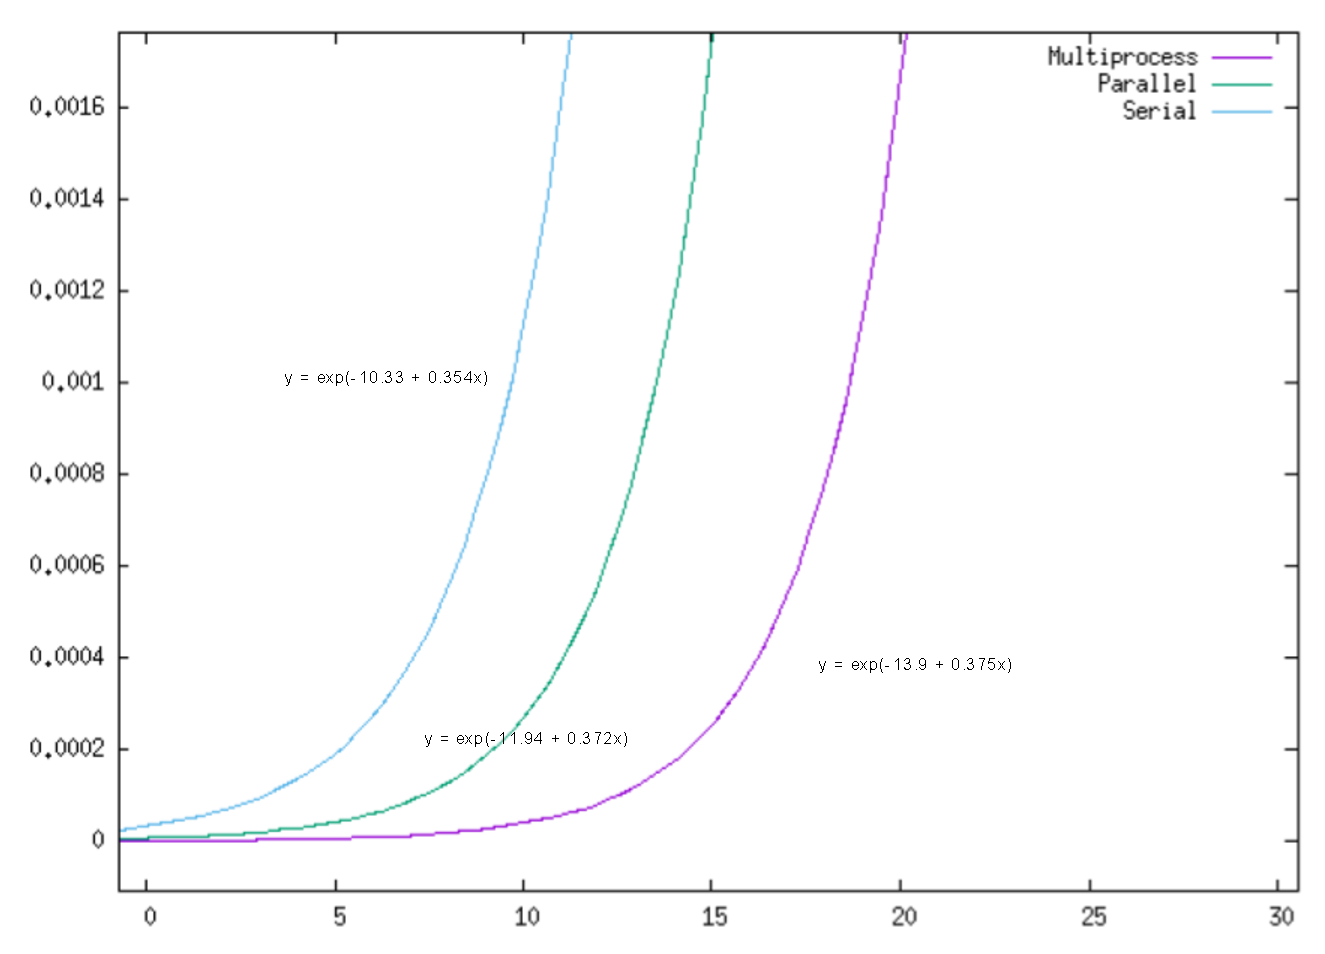
\includegraphics[scale=0.6, bb=0 0 515 478]{figuras/pollard_formulas.eps}
\caption{Equações dos algoritmos de Pollard-rho}
\label{eq_graph}
\end{figure}

Com essas equações, é possível obter o tempo aproximado em segundos para ``quebrar'' uma curva de \(n\) \textit{bits} utilizando os algoritmos implementados. Por exemplo, para saber quanto tempo o algoritmo Pollard-rho serial levaria para ``quebrar'' uma curva de 80 \textit{bits}, basta substituir na fórmula obtida para essa algoritmo
\begin{equation*}
	y = e^{-10.33 + 0.354*80}
\end{equation*}
o valor obtido é \(y = 65006641.53\) segundos, ou seja, fazendo a conversão para dias, levariam 752.39 dias (cerca de 2 anos) para quebrar uma curva de 80 \textit{bits} com o algoritmo Pollard-rho serial e com as configurações de \textit{hardware} utilizadas.

O gráfico da Figura \ref{eq_graph} permite visualizar melhor o comportamento dos algoritmos. Pode-se perceber que a curva do algoritmo serial é a que cresce mais rapidamente, ou seja, este algoritmo necessitará de mais tempo para ``quebrar'' a curva do que os demais.

Outro experimento realizado foi medir o desempenho do algoritmo Pollard-rho multiprocessado em função da quantidade de processadores (\textit{cores}). Para isso, foi selecionada uma curva de 48 \textit{bits}. Os testes foram realizados com a quantidade de processadores indo de um até sete, pois um dos \textit{cores} está reservada para o processo servidor. Os resultados estão descritos na tabela \ref{table:results_mproc}.

\begin{table}[h]
\centering
\begin{tabular}{|c|c|c|c|c|c|c|}
\hline
\rowcolor[gray]{0.9}
\textbf{1 core}  & \textbf{2 cores} & \textbf{3 cores} & \textbf{4 cores} & \textbf{5 cores} & \textbf{6 cores} & \textbf{7 cores} \\ \hline
2m47s    & 5m20s   & 5m35s   & 6m32s   & 2m27s   & 2m15s   & 1m37s   \\ \hline
8m35s    & 3m16s   & 7m14s   & 2m44s   & 1m53s   & 2m22s   & 3m58s   \\ \hline
7m12s    & 5m13s   & 2m37s   & 3m23s   & 3m20s   & 3m03s   & 0m12s   \\ \hline
11m25s   & 3m26s   & 5m55s   & 4m55s   & 1m11s   & 4m38s   & 1m59s   \\ \hline
3m07s    & 2m30s   & 3m42s   & 4m01s   & 0m46s   & 1m45s   & 3m46s   \\ \hline
3m13s    & 1m37s   & 4m01s   & 6m44s   & 0m19s   & 4m01s   & 4m02s   \\ \hline
1m42s    & 6m36s   & 3m41s   & 2m22s   & 5m18s   & 2m00s   & 3m22s   \\ \hline
8m31s    & 4m25s   & 1m16s   & 4m39s   & 5m30s   & 2m06s   & 1m50s   \\ \hline
9m34s    & 5m32s   & 7m14s   & 1m07s   & 6m57s   & 2m59s   & 2m10s   \\ \hline
10m31s   & 4m47s   & 6m49s   & 5m32s   & 3m51s   & 4m18s   & 1m07s   \\ \hline
\end{tabular}
\caption{Resultado dos algoritmos Pollard-rho multiprocessado para quantidades diferentes de processadores}
\label{table:results_mproc}
\end{table}

Calculando-se a média aritmética, a variância e o desvio-padrão para os valores da tabela \ref{table:results_mproc} obtém-se os valores da tabela \ref{table:estatistica_mproc}.

\begin{table}[h]
\centering
\begin{tabular}{|l|c|c|c|}
\hline
\rowcolor[gray]{0.9}
\multicolumn{1}{|c|}{\textbf{Cores}} & \textbf{Média aritmética}  & \textbf{Variância} & \textbf{Desvio-padrão} \\ \hline
1                                    & 399.7                      & 46971.34           & 216.73                 \\ \hline
2                                    & 256.6                      & 8496.04            & 92.17                  \\ \hline
3                                    & 288.4                      & 15236.49           & 123.44                 \\ \hline
4                                    & 252.1                      & 11981.88           & 109.46                 \\ \hline
5                                    & 189.2                      & 17911.51           & 133.83                 \\ \hline
6                                    & 176.9                      & 3864.99            &  62.17                 \\ \hline
7                                    & 144.3                      & 6229.57            &  78.93                 \\ \hline
\end{tabular}
\caption{Valores algoritmo Pollard-rho multiprocessado para quantidades diferentes de processadores}
\label{table:estatistica_mproc}
\end{table}

Observando os dados da tabela \ref{table:estatistica_mproc}, pode-se observar que existe uma melhoria de desempenho quando em função da quantidade de processadores utilizados. É possível perceber também que, com uma quantidade maior de processadores, o desvio-padrão diminui, ou seja, os dados dos testes não tiveram variações abruptas em relação à média. Os testes utilizando apenas um processador (\textit{core}) foi o teste que apresentou maior variação em torno da média, por isso, teve o maior desvio padrão. Inclusive este caso é mais lento que o algoritmo serial, pois nem todos os pontos são considerados, apenas os pontos considerados distintos. Os testes utilizando dois processadores apresentaram uma média de tempo menor do que os testes utilizando três processadores, porém o desvio padrão para três processadores foi maior, o que indica que tem que alguns testes apresentaram resultados mais distantes da média esperada.

É importante saber que na geração dos resultados deste trabalho foi possível utilizar apenas uma máquina para a execução dos algoritmos, o que garante que as características de hardware utilizadas foram as mesmas, porém essa medida acaba comprometendo bastante tempo do cronograma. Até porque foram executados ao menos quatro vezes a mesma curva, por conta da característica do algoritmo que seleciona um ponto inicial de forma aleatória a cada nova execução. Os resultados da tabela \ref{table:results} mostram valores referentes à média dos tempos coletados para os valores de \textit{bits}.
